\begin{frame}{A pathological problem example}


An input sequence:

\vspace{1em}

\begin{tabular}{|c|c|c|c|c|c|c|c|c|c}
	\hline  marker & 0&  1&  0&  $\hdots$& 0 & 1 & 0 & 0  \\ 
	  value & 0.3&  \textbf{0.7}&  0.1&  $\hdots$& 0.2& \textbf{0.4} & 0.6& 0.9  \\ 
	\hline 
\end{tabular}

\vspace{1em}
The predicted output should be the sum of the two one marked positions (1.1). 
\pause
\vspace{1em}
\begin{block}{Why is this a difficult problem?}
	\pause
	Because of it's long time dependencies.
\end{block}

\end{frame}

\begin{frame}{Unfolding}
	\tikzstyle{rnn_style}=[->,shorten >=1pt,auto,node distance=1.5cm,
	thick,
	neuron/.style={circle,fill=white!50,draw,minimum size=0.7cm,font=\sffamily\Large\bfseries},
	missing/.style={circle,fill=white!50,draw=none,minimum size=0.7cm,font=\sffamily\Huge\bfseries},
	label/.style={node distance=1.2cm,rectangle,fill=white!50,draw=none,minimum size=0.7cm,font=\sffamily\normalsize},
	layer/.style={rectangle,fill=white!50,draw,minimum width=4cm,font=\sffamily\normalsize},
	loopStyle/.style={in=120,out=60, distance=2.5cm},]
	

		
	\begin{figure}[h!]
		\centering
		\resizebox{8cm}{!}{
		\begin{tikzpicture}[rnn_style]
		
		%t=0
		\node[layer] (hl1) {Hidden layer t=0};
		
		\node[neuron]    (x0)[below left=0.3cm and 1cm of hl1]       {};
		\node[label]    (u0)[left of=x0]   {$\vec{u}_1$};
		
		
		
		\node[neuron] (o0) [above right=0.3cm and 1cm of hl1] {};
		\node[label]    (y0)[right of=o0]   {$\vec{y}_1$};
		
		%t=1
		\node[layer] (hl2)[above of=hl1,node distance=2.5cm] {Hidden layer t=1};
		
		\node[neuron]    (x1)[below left=0.3cm and 1cm of hl2]      {};
		\node[label]    (u1)[left of=x1]   {$\vec{u}_2$};
		
		
		\node[neuron] (o1) [above right=0.3cm and 1cm of hl2] {};
		\node[label]    (y1)[right of=o1]   {$\vec{y}_2$};
		
		%dots
		\node[label,font=\sffamily\Huge\bfseries] (hld)[above of=hl2,node distance=2cm] {$\hdots$};
		
		%t=T
		\node[layer] (hlT)[above of=hld,node distance=2cm] {Hidden layer t=T};
		
		\node[neuron]    (xT)[below left=0.3cm and 1cm of hlT]      {};
		\node[label]    (uT)[left of=xT]   {$\vec{u}_T$};
		
		
		\node[neuron] (oT) [above right=0.3cm and 1cm of  hlT] {};
		\node[label]    (yT)[right of=oT]   {$\vec{y}_T$};
		
		
		%biases
		\node[neuron](b) [right of=y1,node distance=1.4cm] {};
		\node[label] (b_l) [above of=b,node distance=0.7cm] {bias=1};
		
		
		\path[->] (x0) edge [bend right] node[]{$W^{in}$}   (hl1)
		(u0) edge []   (x0)
		(o0) edge []   (y0)
		(x1) edge [bend right] node[]{$W^{in}$} (hl2)
		(u1) edge []   (x1)
		(o1) edge []   (y1)
		(xT) edge [bend right] node[]{$W^{in}$} (hlT)
		(uT) edge []   (xT)
		(oT) edge []   (yT)
		
		
		(hl1) edge [bend left]  node[]{$W^{out}$} (o0)
		(hl2) edge [bend left]  node[]{$W^{out}$} (o1)
		(hlT) edge [bend left]  node[]{$W^{out}$} (oT)
		
		(b)  edge [bend left,dotted,in = 90]  node[]{$b^{out}$} (o0)
		(b)  edge [bend left, dotted, in = 90,out=80]  node[]{$b^{rec}$} (hl1)
		(b)  edge [bend left, dotted]  node[]{$b^{rec}$} (hl2)
		(b)  edge [bend left,dotted]  node[]{$b^{out}$} (o1)
		(b)  edge [bend left, dotted,in = 200]  node[]{$b^{rec}$} (hlT)
		(b)  edge [bend left,dotted,in =200]  node[]{$b^{out}$} (oT)
		(hl1) edge [] node[]{$W^{rec} $} (hl2)
		(hl2) edge [] node[]{$W^{rec} $} (hld)
		(hld) edge [] node[]{$W^{rec} $} (hlT);
		
		\end{tikzpicture}
	}
		\caption{Unfolding of a $\net{RNN}$}
		\label{rnn_unfolding}
	\end{figure}
\end{frame}

\begin{frame}{Understanding the gradient structure}
	Simply applying the chain rule it's easy to see that
	\begin{equation}
		\nabla L(\vec{x}) = \sum_{t=1}^T \nabla L_{|t}(\vec{x}),
	\end{equation}
	where $\nabla L_{|t}$ is ...
\end{frame}

\begin{frame}{Vanishing gradient: an upper bound}
	\begin{equation}
	\frac{\partial \vec{a}^t}{\partial \vec{a}^k} = \prod_{i=t-1}^{k}  diag(\sigma'(\vec{a}^i)) \cdot \mat{W}^{rec}.
	\label{eq:temporalComponent}
	\end{equation}
	
	Taking the singular value decomposition of $\mat{W}^{rec}$:
	\begin{equation}
	\mat{W}^{rec} =  \mat{S}\cdot\mat{D}\cdot\mat{V}^T
	\end{equation}
	where $\mat{S},\mat{V}^T$ are squared orthogonal matrices and $\mat{D}\defeq diag(\mu_1, \mu_2,...,\mu_r)$ is the diagonal matrix containing the singular values of $\mat{W}^{rec}$.
	Hence:
	\begin{equation}
	\frac{\partial \vec{a}^t}{\partial \vec{a}^k} = \prod_{i=t-1}^{k}  diag(\sigma'(\vec{a}^i)) \cdot \mat{S}\cdot \mat{D} \cdot \mat{V}^T
	\end{equation}
	\end{frame}
	\begin{frame}
			Since $\mat{U}$ and $\mat{V}$ are orthogonal matrix, hence $$\norm{\mat{U}}_2=\norm{\mat{V}^T}_2 = 1,$$ and $$\norm{diag(\lambda_1, \lambda_2,...,\lambda_r)}_2 \leq \lambda_{max},$$ we get
			\begin{align}
			\norm{\frac{\partial \vec{a}^t}{\partial \vec{a}^k}}_2 &= \norm{ (\prod_{i=t-1}^{k} diag(\sigma'(\vec{a}^i)) \cdot \mat{S}\cdot \mat{D} \cdot \mat{V}^T)}_2\\
			&\leq (\sigma'_{max} \cdot \mu_{max})^{t-k-1}
			\end{align}
	\end{frame}



\begin{frame}{Temporal gradient norms: an illustration}
\begin{figure}
	\centering
	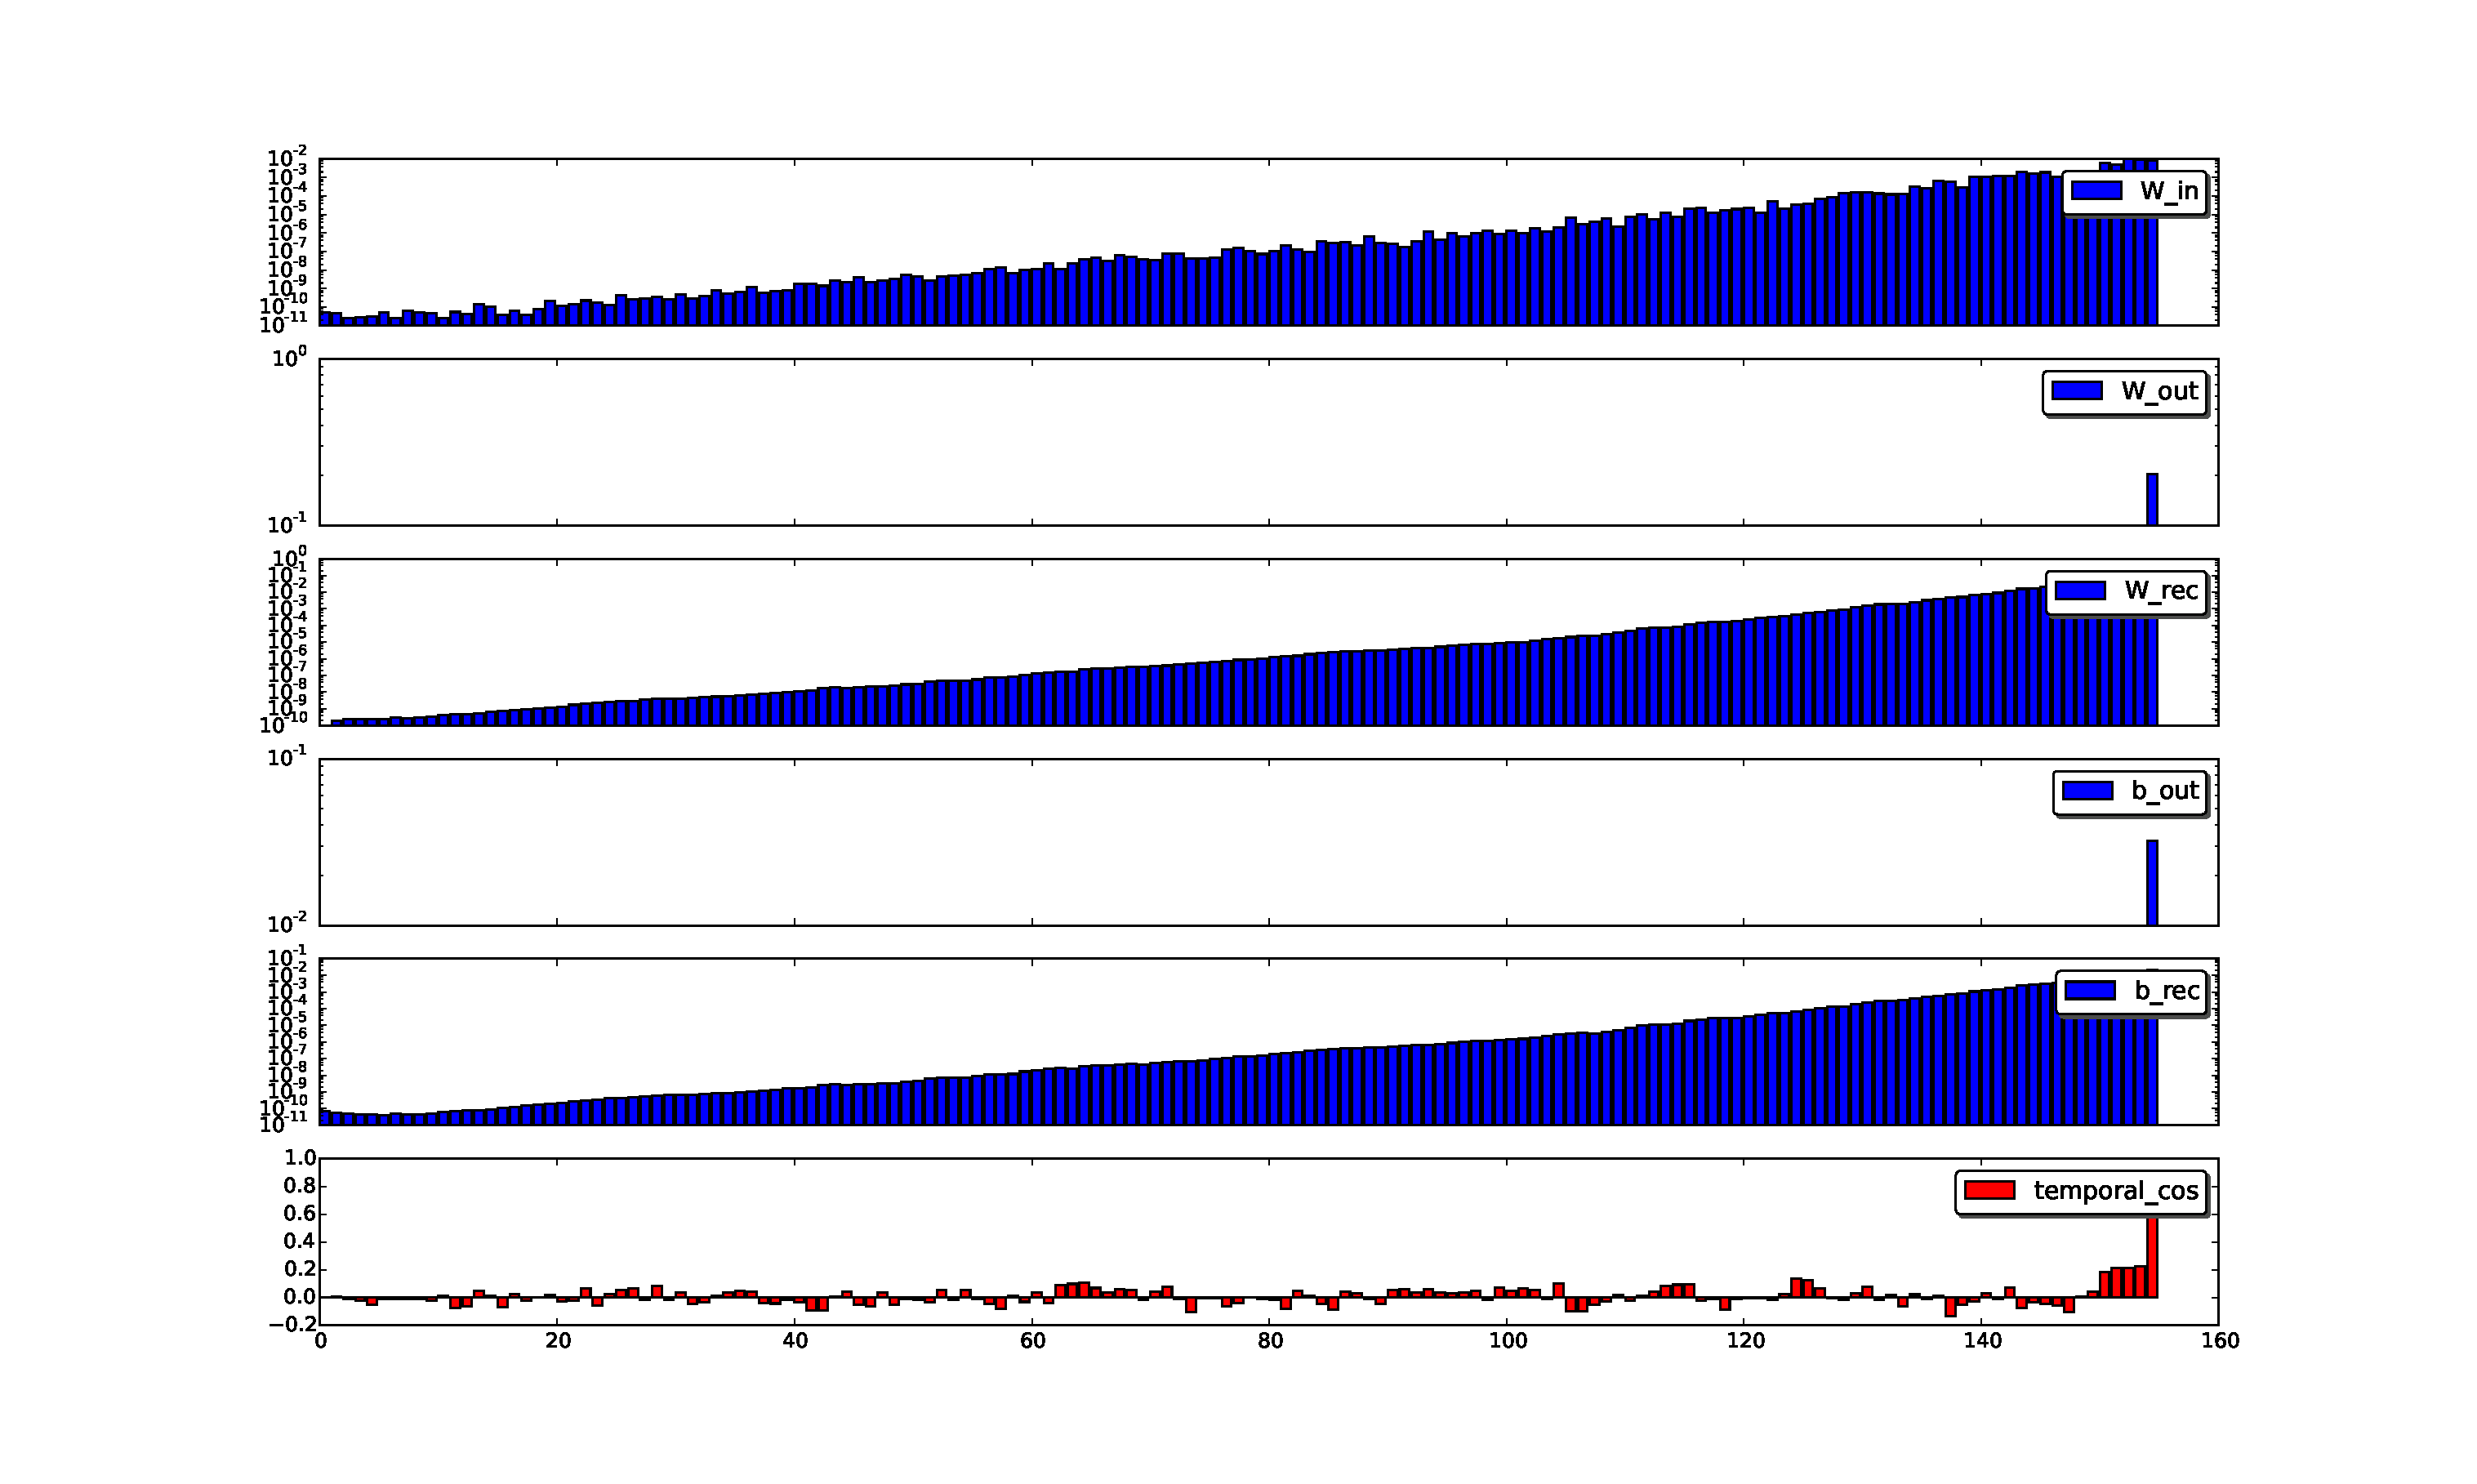
\includegraphics[width=1\textwidth]{temporal_gradients.eps}
\end{figure}
\end{frame}

